\section{Ausgangslage und Erweiterungen}
\label{sec:Ausgangslage und Erweiterungen}

\paragraph{Projekt 5}\mbox{}

Das Projekt 5 hat die Basis für das Projekt 6 gebildet. In diesem wurde ein Konzept erarbeitet, welches die Hauptkomponenten der Maschine festlegte und deren Arbeitsweise. Durch diese Konzepterstellung war es möglich ein Blockschaltbild zu erstellen, welches diese Komponenten im Groben zusammen vereinte. Zu den Systemen zählten dabei: 

\begin{itemize}
\item Pumpen zur Beförderung der Flüssigkeiten
\item Durchflussmessgeräte zur Dosierung der Flüssigkeiten
\item Ein Motor, welcher ein Glas befördern soll
\item Ein Display, über welches die Maschine bedient werden kann
\end{itemize}
\mbox{}

Nach der Auswahl dieser Hauptkomponenten konnte dann die Ansteuerung theoretisch aufgebaut werden. Dazu gehörten folgende Komponenten:

\begin{itemize}
\item Ein Mikrocontroller, welcher die Software beinhaltet und alle für die Ansteuerungen benötigten Schnittstellen bietet 
\item Eine 48V-Spannungsquelle zur Speisung des Motors
\item Eine 12V-Spannungsquelle zur Speisung der Pumpen
\item Eine 5V-Spannungsquelle zur Speisung des Mikrocontrollers, der Durchflussmessgeräte und des Displays
\item Eine 3.3V-Spannungsquelle zur Speisung der Motorenansteuerung
\end{itemize}
\mbox{}

Ein weiterer Teil des Projekt 5 war es, die gewählten Komponenten und die daraus entstandenen Teilsysteme in einem Testaufbau aufzubauen und zu evaluieren. Der Mikrocontroller wurde im Projekt 5 so ausgewählt, dass es möglich war weitere Komponenten anzubinden. 

\paragraph{Projekt 6}\mbox{}

Das im Projekt 5 entstandene Blockschaltbild ist nun im Projekt 6 um weitere Teilsysteme ergänzt worden, was in Abbildung \ref{fig:Blockschaltbild_Partymixer} zu sehen ist. Auf diese Teilsysteme wird mit den vorherigen Teilsystemen detailliert im Kapitel \ref{sec:Printaufbau} und \ref{sec:Teilsysteme} eingegangen. Zu den neuen Systemen gehören die grün umrahmten Teilsysteme. Die Erweiterungen bestehen aus:

\begin{itemize}
\item Ein Wireless-/Bluetoothmodul, welches eine externe Ansteuerung per Web-Server oder Android App ermöglicht und eine dazugehörige Programmierschnittstelle 
\item Einem RFID Lesegerät
\item Einem SD-Karten Slot
\item Einer Maschinenbeleuchtung 
\item Einem ABN-Encoder zur Positionsgebung des Motors
\end{itemize}
\mbox{}



\begin{figure}[h!]
\center
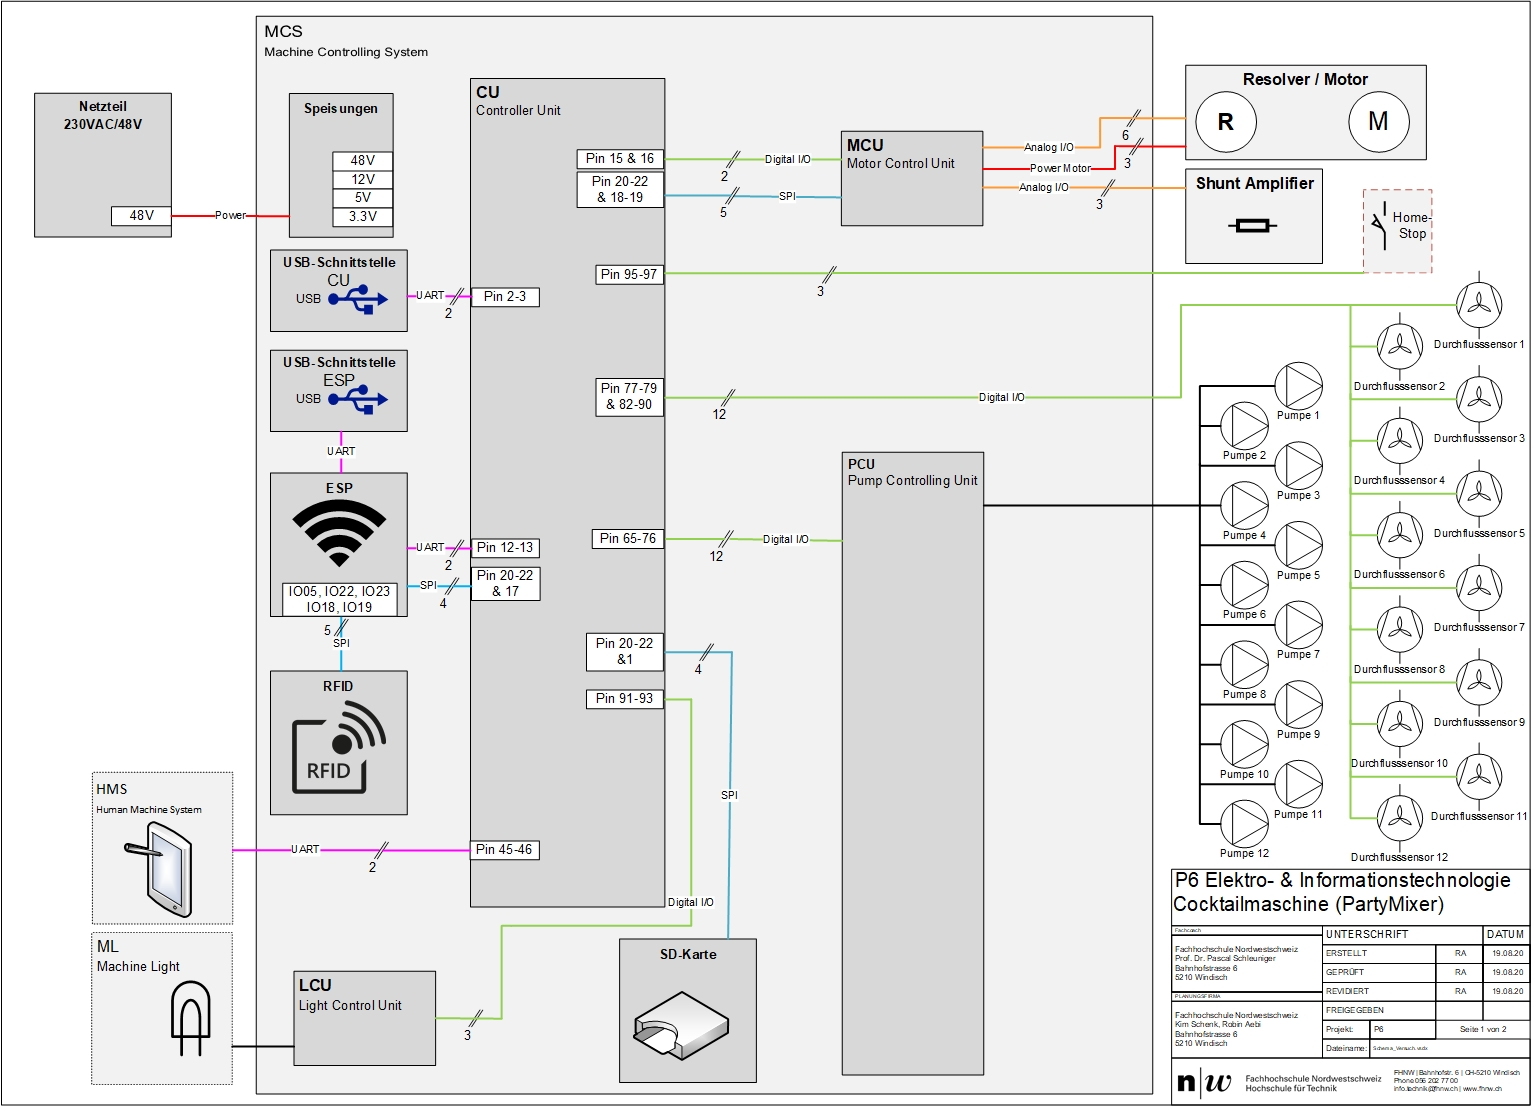
\includegraphics[angle=90, width = \textwidth]{graphics/Blockschaltbild}
\caption{Blockschaltbild des PartyMixer's gemäss Projekt 6.}
\label{fig:Blockschaltbild_Partymixer}
\end{figure}

\newpage

